\problemname{Floor Area}
\noindent
You are soon going to sell your house, but first, you need to figure out the size of the floor area. It might sound easy,
but you have an unused storage room for which you've lost the key, and you have no idea how big the storage room is.
The only thing in the storage room is a robot vacuum cleaner. If you start the vacuum cleaner and see where
it ends up, maybe you can figure out how big the storage room is?

The storage room consists of an $N \times M$ grid, where $N$ and $M$ are unknown positive integers. The rows are
numbered from $0$ to $N-1$ from top to bottom, and the columns are numbered from $0$ to $M-1$ from left to right.
The robot has a list of instructions $s$. The instructions are described by a string consisting of the characters \verb|<|, \verb|>|, \verb|^|, and \verb|v|.
When the robot is started, it reads these instructions, and for each one, it moves one step in the corresponding direction.
If the robot tries to move outside the grid, then it hits a wall and nothing happens.
The robot starts in the upper-left corner, i.e., at row $0$ and column $0$.

You are given the string $s$ and the row and column where the robot ended up after following the instructions.
Calculate the smallest possible value of $N \cdot M$ that is consistent with this information.

\section*{Input}
The first line contains an integer $K$ ($1 \leq K \leq 3 \cdot 10^5$), the length of the string $s$.

The second line contains the string $s$.

The third line contains two integers $r$ and $c$ ($0 \leq r,c < 3 \cdot 10^5$), where
$r$ is the row where the robot ended up, and $c$ is the column where it ended up.

\section*{Output}
Print an integer, the smallest possible value of $N \cdot M$. If there is no choice of $N$ and $M$ consistent
with the information in the test data, then print $-1$ instead.

\section*{Points}
Your solution will be tested on several test case groups.
To get the points for a group, it must pass all the test cases in the group.

\noindent
\begin{tabular}{| l | l | p{12cm} |}
  \hline
  \textbf{Group} & \textbf{Point value} & \textbf{Constraints} \\ \hline
  $1$    & $15$       & The robot only moves down and to the right. \\ \hline
  $2$    & $30$       & $K \leq 100$ \\ \hline
  $3$    & $20$       & $K \leq 5000$ \\ \hline
  $4$    & $35$       & No additional constraints. \\ \hline
\end{tabular}

%\section*{Samples}

\section*{Explanation of sample case}
\begin{centering}
  \begin{figure}[h]
      \centering
      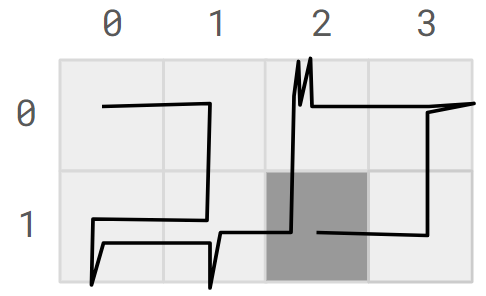
\includegraphics[width=0.4\textwidth]{golvyta.PNG}
      \caption{The picture shows the smallest possible grid in sample case 1.
      The robot travels according to the black curve.
      The dark square is the robot's final position.}
      \label{fig:enter-label}
  \end{figure}
\end{centering}
